\documentclass[a5paper, 12pt]{book}
\usepackage{geometry}

%enumerate kann man dann anpassen
\usepackage{enumerate}
%Um Bilder einzufügen
\usepackage{graphicx}
%um subfigures zu erstellen, damit ich mehrere bilder zu einer figure zusammenfügen kann
\usepackage{caption}
\usepackage{subcaption}
\usepackage{hyperref}
\usepackage{anyfontsize}
\usepackage{textcomp}

%SubSubsections werden gezählt
\setcounter{tocdepth}{3}
\setcounter{secnumdepth}{3}

\geometry{a5paper, total = {4in,5in}}

\newcommand{\neueregel}{
\noindent Regel, die geändert oder hinzugefügt werden soll:

\vspace{2cm}
\noindent Was soll geändert/hinzugefügt werden?

\vspace{13cm}
Antragsteller:
\newpage
}
\newcommand{\twoemptypages}{
\thispagestyle{plain}
\mbox{}
\newpage
\thispagestyle{plain}
\mbox{}
\newpage
}


\begin {document}
\renewcommand{\listfigurename}{Abbildungs- verzeichnis}
\pagenumbering{gobble}
\newgeometry{top=6cm, total = {4in,5in}}
\begin{titlepage}
\begin{center}
{\fontsize{40}{48}\selectfont \textbf{Wal-BGB}\par}

\begin{large}
\vspace{0.3cm}
The great Beerpong rulebook\\
\vspace{1cm}
Smion Schweiger Schweiger\\
translation strongly aided by ChatGPT\\
\vspace{1cm}
based on the third version from october 2025
\end{large}
\end{center}
\vspace{6cm}

\end{titlepage}

\begin{center}
\vspace*{2.5cm}
\scalebox{3.5}{\S 420}
\par
\smallskip
\large{In doubt a Wal-WG\texttrademark-member is always right.}\label{Vorwort}
\end{center}
\restoregeometry
\pagebreak
\begin{Large} \textbf{Preface\\}
\end{Large}
This book was created to provide the Beer Pong games in the Wal-WG™ with a solid set of rules and to eliminate any remaining uncertainties. However, since the author is not a lawyer but merely a lousy teacher trainee, there will certainly still be various mistakes, even after quite a few have been corrected for the 3rd edition. There is a section in the appendix where notes about gaps in the rules, logical inconsistencies, or similar issues can be made. Other comments and suggestions are also welcome, as long as they somehow relate to Beer Pong.\\
There is a major rule change for the third edition: players can now decide at the beginning of the game whether they want to rearrange on even or odd cup counts. Another entirely new rule is that, in addition to being onFire, players can now also be onIce. Furthermore, there were many small adjustments that improve the precision of the interpretations.
In the third edition, several formatting changes were made. The two most important ones are the use of the generic feminine form and the \texttrademark. A complete list of all changes can be found in the patch notes (\ref{chap:patchnotes}).\\
New features include the introduction of a Beer Pong Elo rating, as well as this English rulebook.
Thanks go out to all the people who have already played Beer Pong matches in the Wal-WG™ and thus laid the foundation for the development of this rule set. Further thanks to Vinne, who created all the lovely illustrations and the cover for the third edition, and to everyone who took the time to proofread the fun.\\\\
Thanks also go out to everyone who provided input for necessary rule changes, or simply played games that pushed the previous editions to their limits.
I hope that this rather formal rulebook does not overthink the game – after all, we all just want to get drunk.

\tableofcontents
\cleardoublepage
\pagenumbering{arabic}
\part {Rules}\label{part:regeln}
\chapter*{Rule Violation}\label{chap:regelverstoß}
In the following sections of this rulebook, it is described exactly how a Beer Pong game in the Wal-WG™ is conducted. In some cases, specific penalties are mentioned if certain rules are not followed. For all other rules and principles, it applies that any violation is considered unsportsmanlike and may result in disqualification by a Wal-WG™ member at any time.

\chapter{Definitions}\label{chap:definitionen}

\section{Drinking a Cup}\label{sec:bechertrinken}
When it is stated that cups must be drunk, one player from the team that has to drink must either drink the cup, pour its contents into the cup that is currently being drunk from, or drink the equivalent amount from another vessel (only if this was agreed upon beforehand and the cup originally contained water). In addition, the drunk cup must be placed at the edge of the table. As soon as a team begins to drink from the cup, it no longer counts as one of their cups.  
A cup counts as fully drunk when less than 10 ml of liquid remains inside.

\section{Standard Throw}\label{sec:standardwurf}
A player stands on her own side of the table. She may not position herself on any elevated surface, unless it provides no advantage — for example, if it is clearly farther back.

\section{Trickshot}\label{sec:trickshot}
A trickshot must in some way differ from a standard throw, or be performed in a creative manner toward the opponent’s cups.  
A prerequisite for it to count as a trickshot is that it must be harder to hit than a standard throw (for example, off the wall, backward, space laser, etc.).  
If a trickshot, after being thrown, bounces twice on the table, it may be caught or slapped away by the opposing team.

Throwing with closed eyes or with the weak hand is NOT a trickshot, unless this is explicitly agreed upon.  

The following variations also count as trickshots:

\begin{enumerate} [(1)]
    \item Guest throw: a spectator may execute the throw. She is allowed to perform a standard throw. Since a standard throw is easier to hit than a trickshot, it is considered unsportsmanlike to perform significantly more guest throws than the opposing team (of course in relation to the total number of trickshots per team, not in absolute numbers).

    \item A standard throw made while the thrower is completely naked.
\end{enumerate}

\section{Score}\label{sec:treffer}
A cup counts as scored when one of the following conditions occurs:

\begin{enumerate}
    \item A valid standard throw (see Section \ref{sec:standardwurf}) or trickshot (see Section \ref{subsub:trickshotphase}) lands in a cup and stays there.
    \item A standard throw or trickshot causes a cup to fall over and spill completely.  
    A cup counts as completely spilled when less than 10 ml remain inside. If it is caught or lands upright so that it does not fully spill, it is immediately placed back at the position it stood before falling.  
    Intentionally throwing in such a way that cups are knocked over is considered unsportsmanlike behavior and will not be tolerated in the Wal-WG™.
    \item A team accidentally bounces or throws the ball into one of its own cups in any way.  
    This counts as a score for the opponents but not for any particular player.  
    The only exception is when the ball is thrown to the team to begin their throws.
    \item A player of a team accidentally knocks over one of their own cups, and less than 10 ml remain in it.  
    This counts as a score for the opponents but not for any particular player.
\end{enumerate}

A cup that has been scored under these conditions always also counts as \textit{hit}.  
The term \textit{hit} is used several more times throughout the rulebook and must be clearly distinguished from a \textit{score}.  
For example, during a Bomb (see Section \ref{sec:bombe}), a cup can be marked as hit without being scored.
 
\chapter{Game Setup}\label{chap:spielaufbau}

In Section 2.1, the basic setup of every Beer Pong game in the Wal-WG™ is described.  
As a table, the house-owned beer table must be used, and traditionally, games are played in the bathroom.  
Only table tennis training or competition balls are allowed for throwing.  
Cheap, dentable, whacky Beer Pong balls from Tedi or similar stores are strictly forbidden.  

The game is played with plastic cups holding 0.4 to 0.5 liters.  
Furthermore, for every game, the bathroom door must be removed from its hinges.  

The following figure shows a regular game setup with two beers (each 0.5 liters) per team.  
Alternative variants are possible in which the cups are filled with wine or similar beverages.  
It is theoretically also allowed to fill the cups with water and drink something else (or nothing) —  
however, this is generally frowned upon.  
Any deviation from a regular game must be approved by the opposing team.

\begin{figure}
    \centering
    \begin{subfigure}[h]{0.69\textwidth}
    \centering
    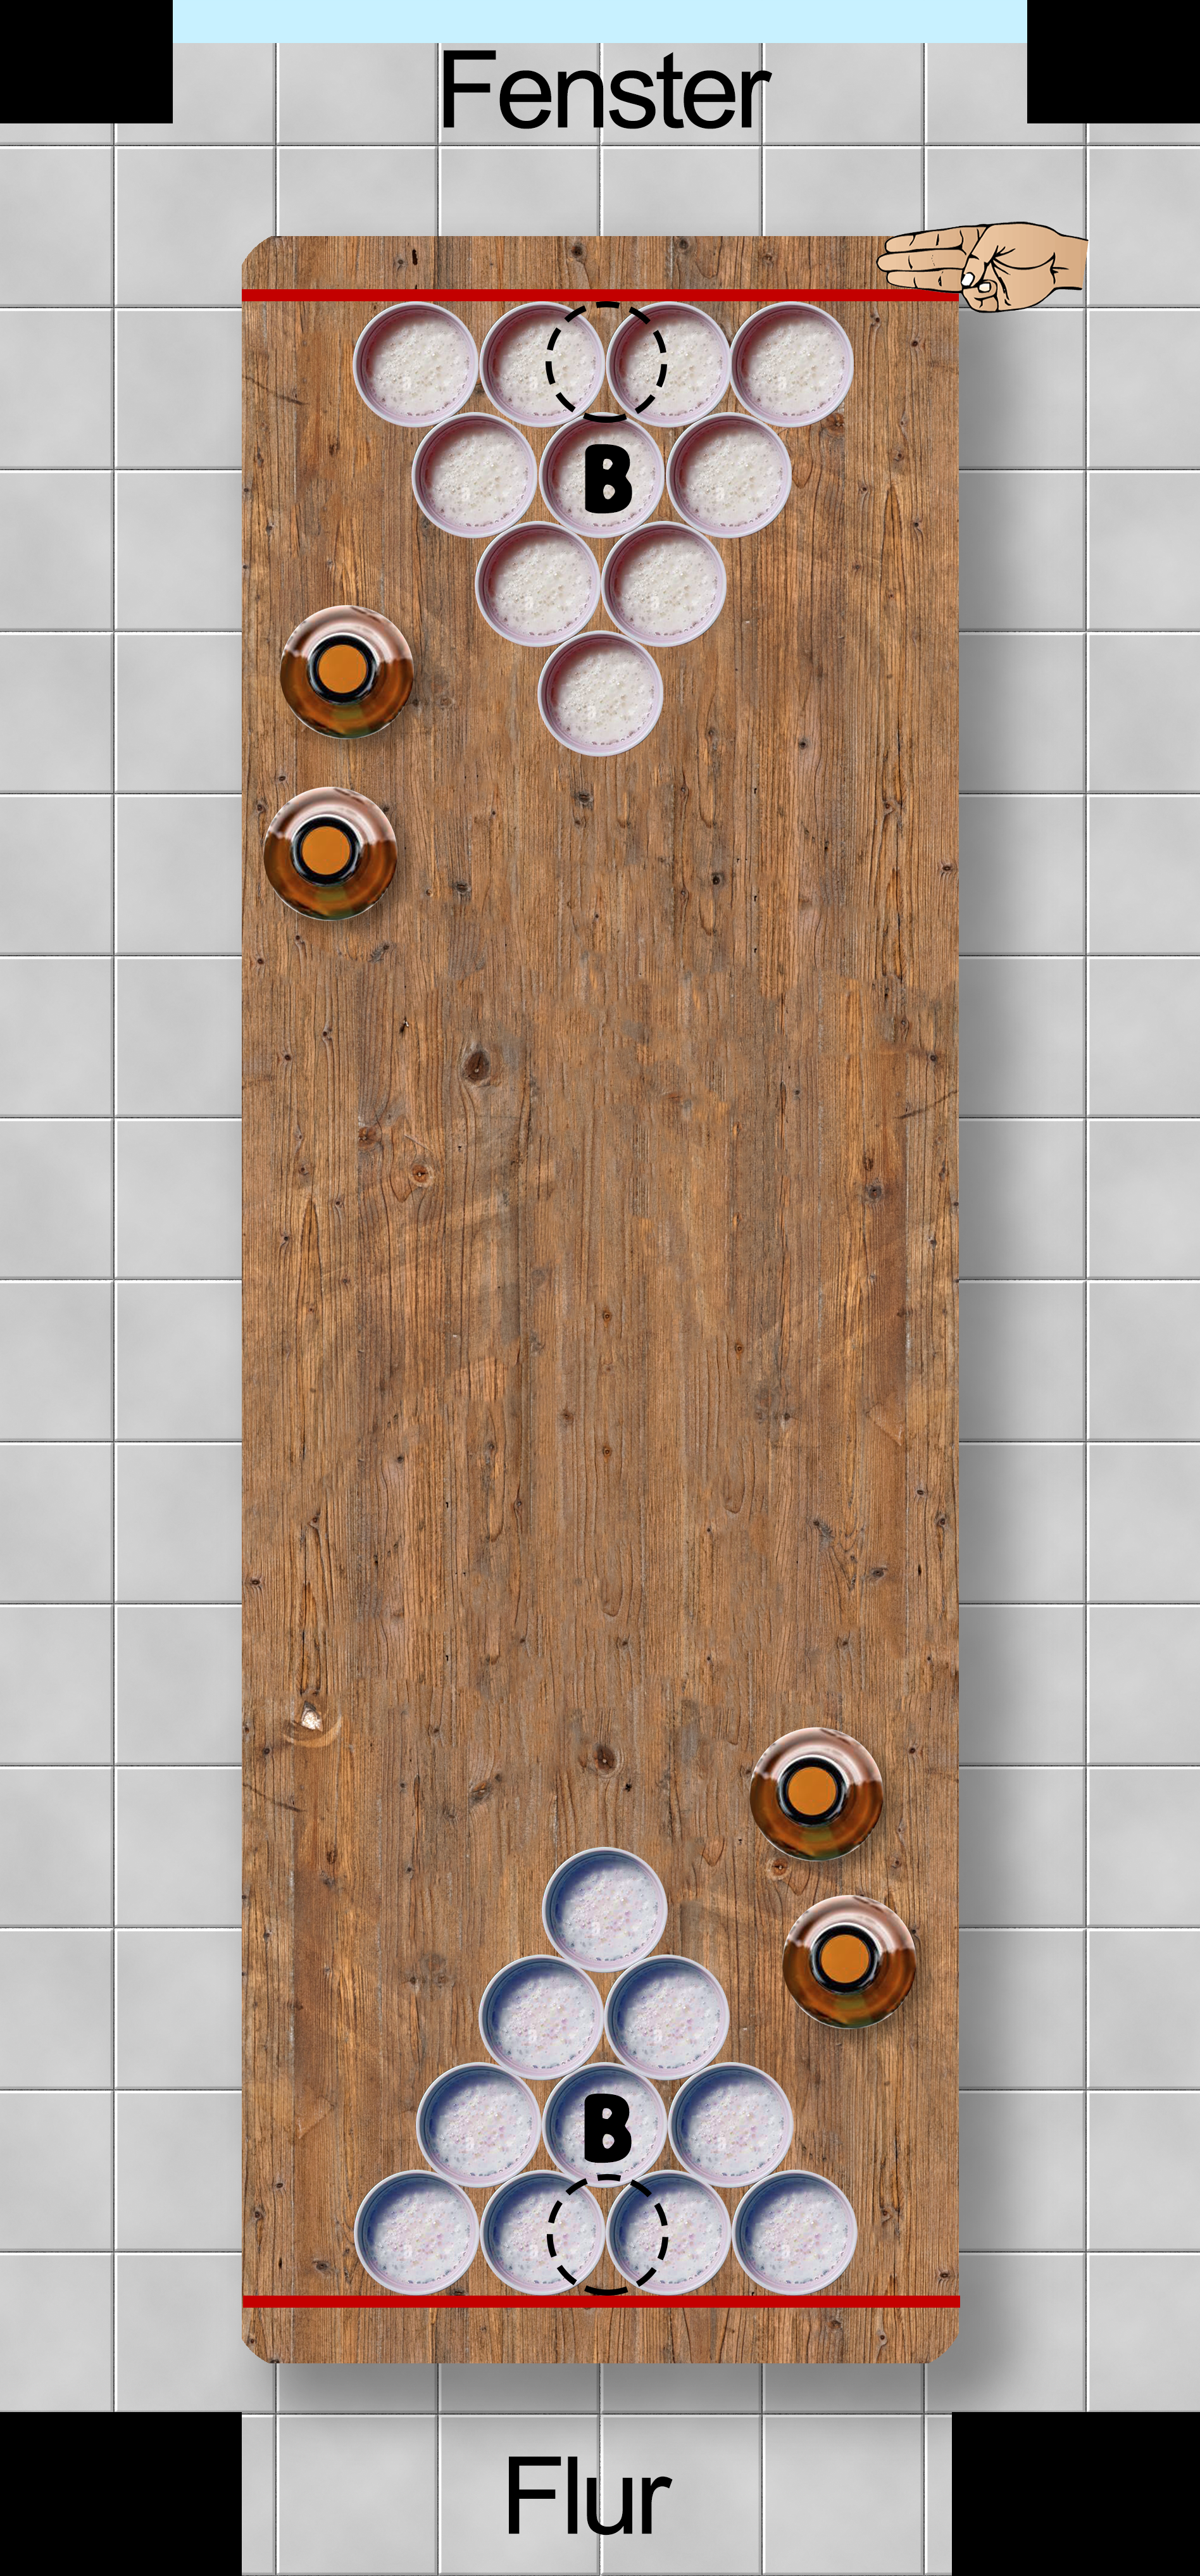
\includegraphics[width=\textwidth]{Grafiken/beerpongregeln_ohne_legende.png}
    \caption{Setup}
    \end{subfigure}
    \hfill
   \begin{subfigure}[h]{0.29\textwidth}
   \centering
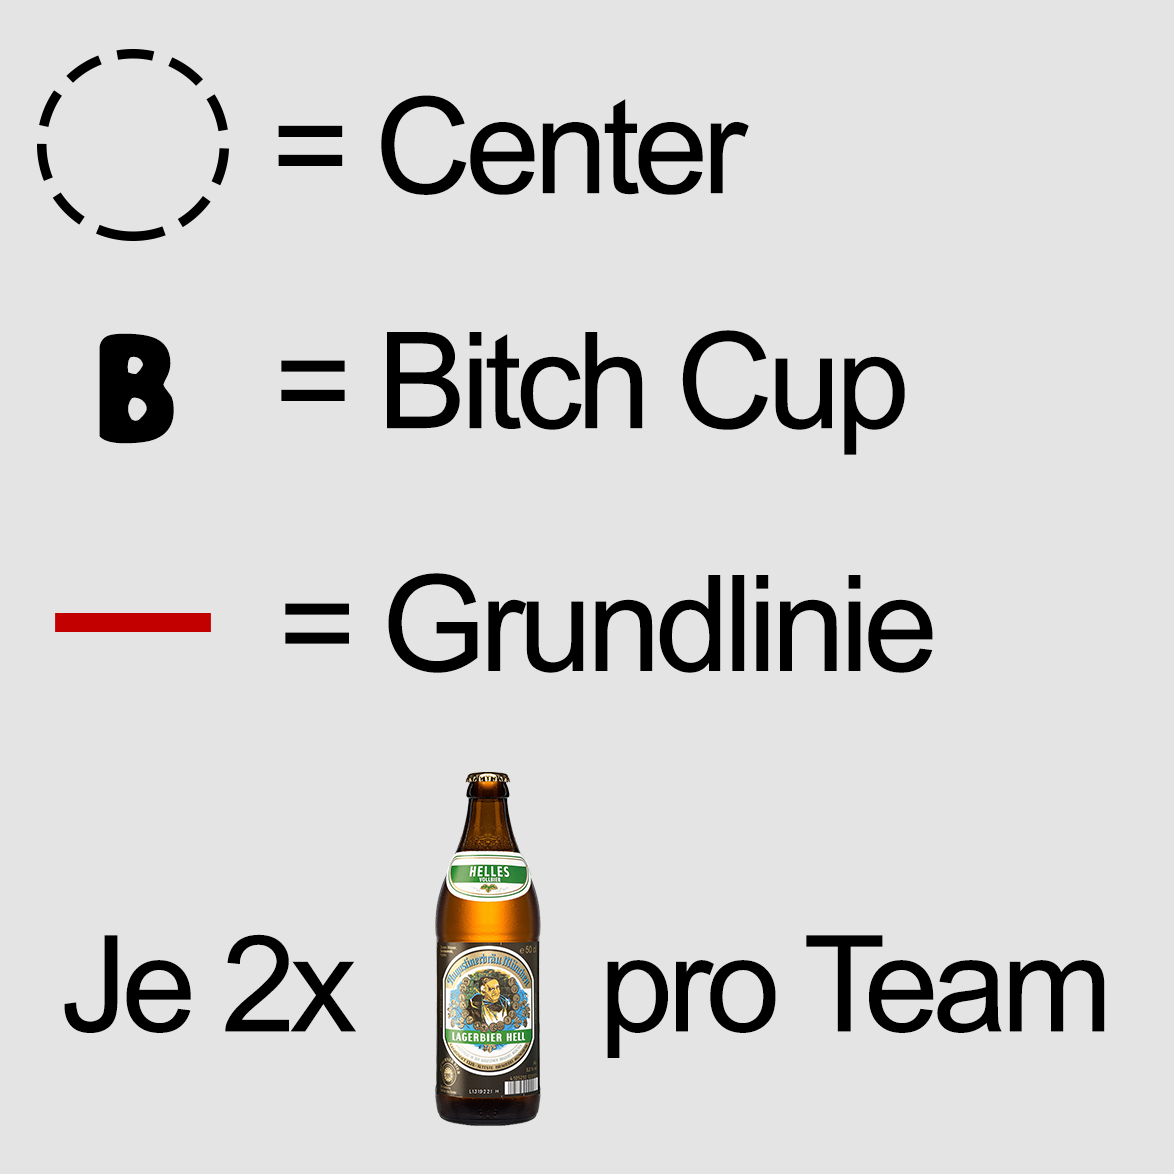
\includegraphics[width=\textwidth]{Grafiken/legende.png}
\caption{Legende}
   \end{subfigure}
    \caption{Game Setup}
    \label{fig:spielaufbau}
\end{figure}


\chapter{Game Procedure}\label{chap:spielablauf}

\section{Sketch of the Game Procedure}
On the next page, a schematic representation shows the rough structure of every Beer Pong game.  
More detailed explanations of each phase follow in the remainder of this chapter.

\begin{figure}[h]
\centering
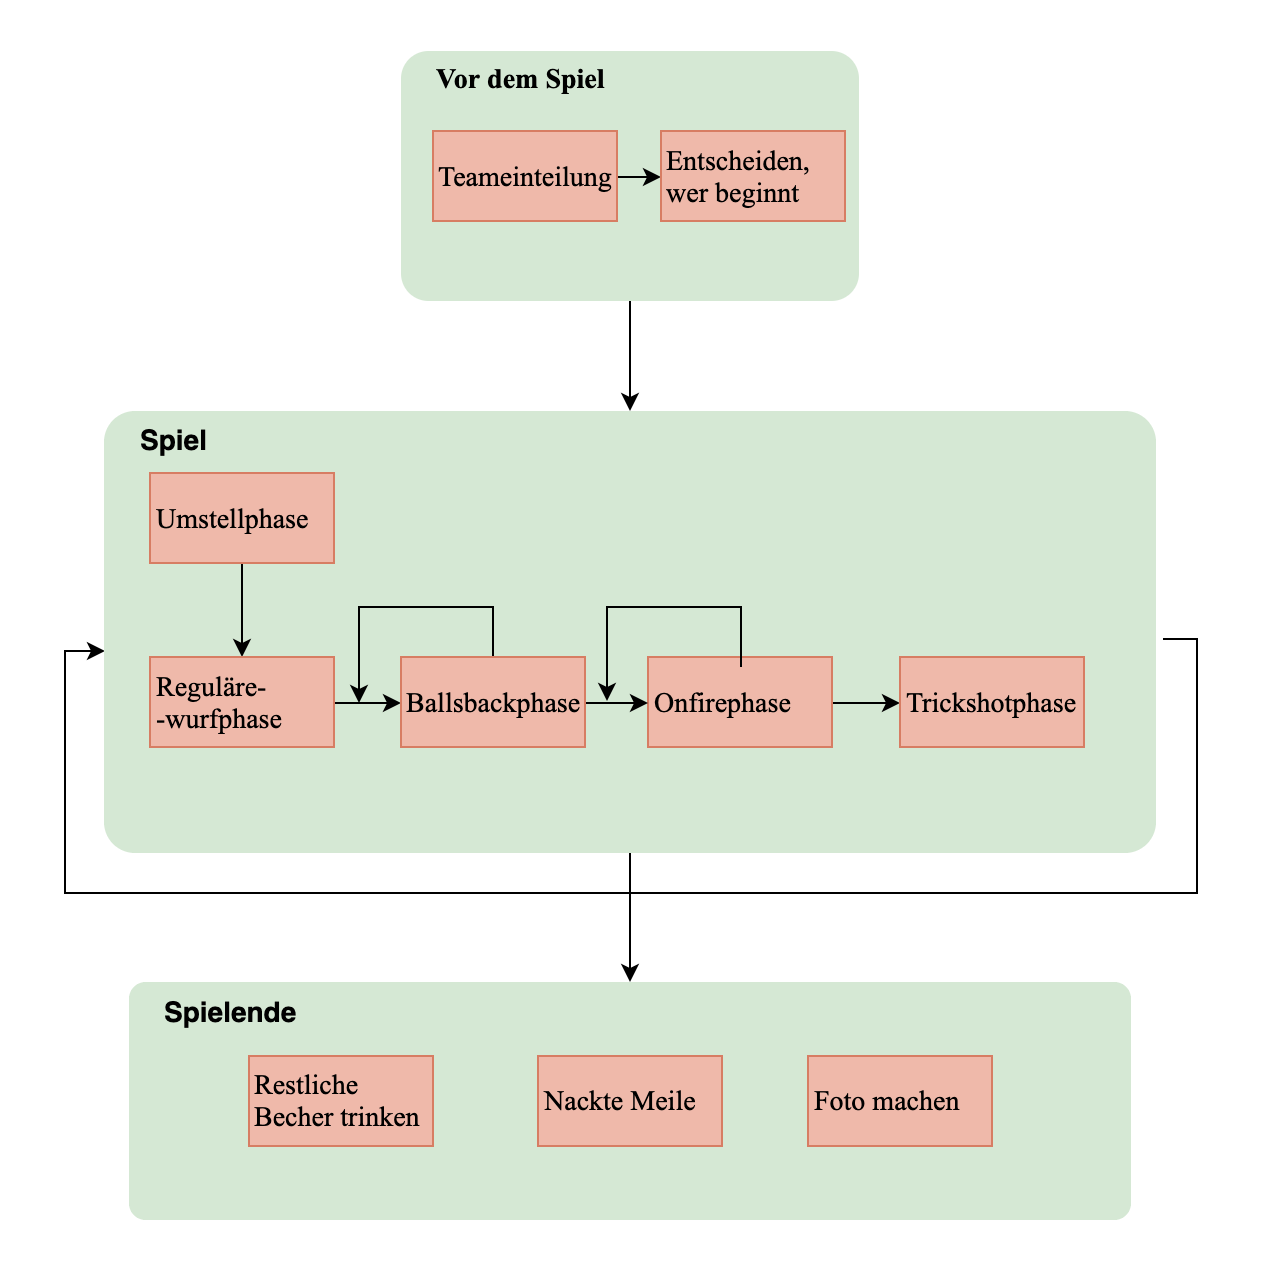
\includegraphics[width=\textwidth]{Grafiken/Bierpongflowneu.png}
\caption{Schematic of the game procedure}
\label{fig:spielablaufskizze}
\end{figure}

\section{Detailed Regulations}\label{sec:genaue_regelungen}

\subsection{Before the Game}

\subsubsection{Team Formation}
Four people who want to play come together.  
To actually be allowed to play, they must first check with everyone else who also wants to play.  
Then they split into teams of two and agree in any freely chosen way on who plays on which side.  
It is also possible to play with any number of people per team.  
The team sizes do not have to be identical.  
However, the principle of the game does not change:  
two balls are still used, and each team always has as many throws per turn as if it consisted of two players.  
If there are more or fewer players, they simply take turns in such a way that everyone throws roughly equally often.

\subsubsection{Side Selection}
Players are free to decide how to determine who plays on which side.  
However, if no agreement can be reached, one round of Rock–Paper–Scissors (without “well”) is played.

\subsubsection{Even or Odd}\label{sec:geradeungerade}
Each team must now decide whether they want to rearrange when there is an even or an odd number of cups remaining in this game.  
This is marked using the indicator attached to the table.  
If this step is forgotten, the currently displayed setting on the table applies.

\subsubsection{Deciding Who Starts} \label{sec:decidewho}
The usual method for determining who starts is called \textit{Eye to Eye}.  
If both parties agree, any other method may also be used.

\paragraph{Eye to Eye:}
Each team selects one team member.  
The selected players stand on their respective sides of the table, look each other in the eyes, and throw simultaneously.  
If one of them scores, her team starts the game.  
If neither or both score, the other two teammates throw next.  
If one of them scores, her team begins the game.  
If neither or both score again, the two players who just threw play a single round of Rock–Paper–Scissors (without “well”).  
The team of the winner starts the game.  

The team that starts begins the game in the \textit{Rearrangement Phase}.  
If, during any of the throws, the balls collide in midair, the two throwers must kiss.

\subsection{Game}\label{subsec:spiel}

The game consists of the Rearrangement Phase and four Throw Phases.

During the Rearrangement Phase, the formation of the opponent’s cups can be modified.

In each Throw Phase, Hits are collected.  
When a phase ends, all cups that have been hit must be drunk.  
In particular, cups must also be drunk if a phase restarts (relevant for BallsBack \ref{sec:ballsback} and OnFire \ref{sec:onfire}).  

An exception applies if the last cup counts as hit — then, after the end of the phase, only all cups except the last one are drunk.  
The team that would normally have to drink that cup then has a chance for Redemption in its next Throw Phases (see Section \ref{sec:redemption}).

Once a team has completed its Trickshot Phase, a round is finished and the other team starts the next round with its Rearrangement Phase, unless the game has already ended.

\subsubsection{Rearrangement Phase}\label{sec:umstellphase}

During the Rearrangement Phase, the active team has two options:

\begin{enumerate}
    \item \textbf{Rearrange:}  
    Each team may rearrange the opponent’s cups once per game.  
    This is only possible when the opponent currently has an even or odd number of cups (as individually decided at the start of the match, see \ref{sec:geradeungerade}).  
    For this, the opponent must be told which formation to set up.  
    Each group of cups must have at least one contact point with the base line.  
    Examples can be seen in Figures \ref{fig:beispielezudenerlaubtenStellungen} and \ref{fig:beispielezudennichterlaubtenStellungen}.
    
    If the formation called “Die Enge Muschi” (see \ref{fig:enge-Muschi}) is to be set, one must explicitly request “die Enge Muschi”  
    With vague descriptions such as “the tight one” or “the offensive diamond,” the team required to move their cups may act as if they did not hear it.
    
    \item \textbf{Centering:}  
    If the opponents have only one cup left, one may demand that they place it in the center position (see Figures 3.3 and 3.4).
\end{enumerate}
\begin{figure} 
    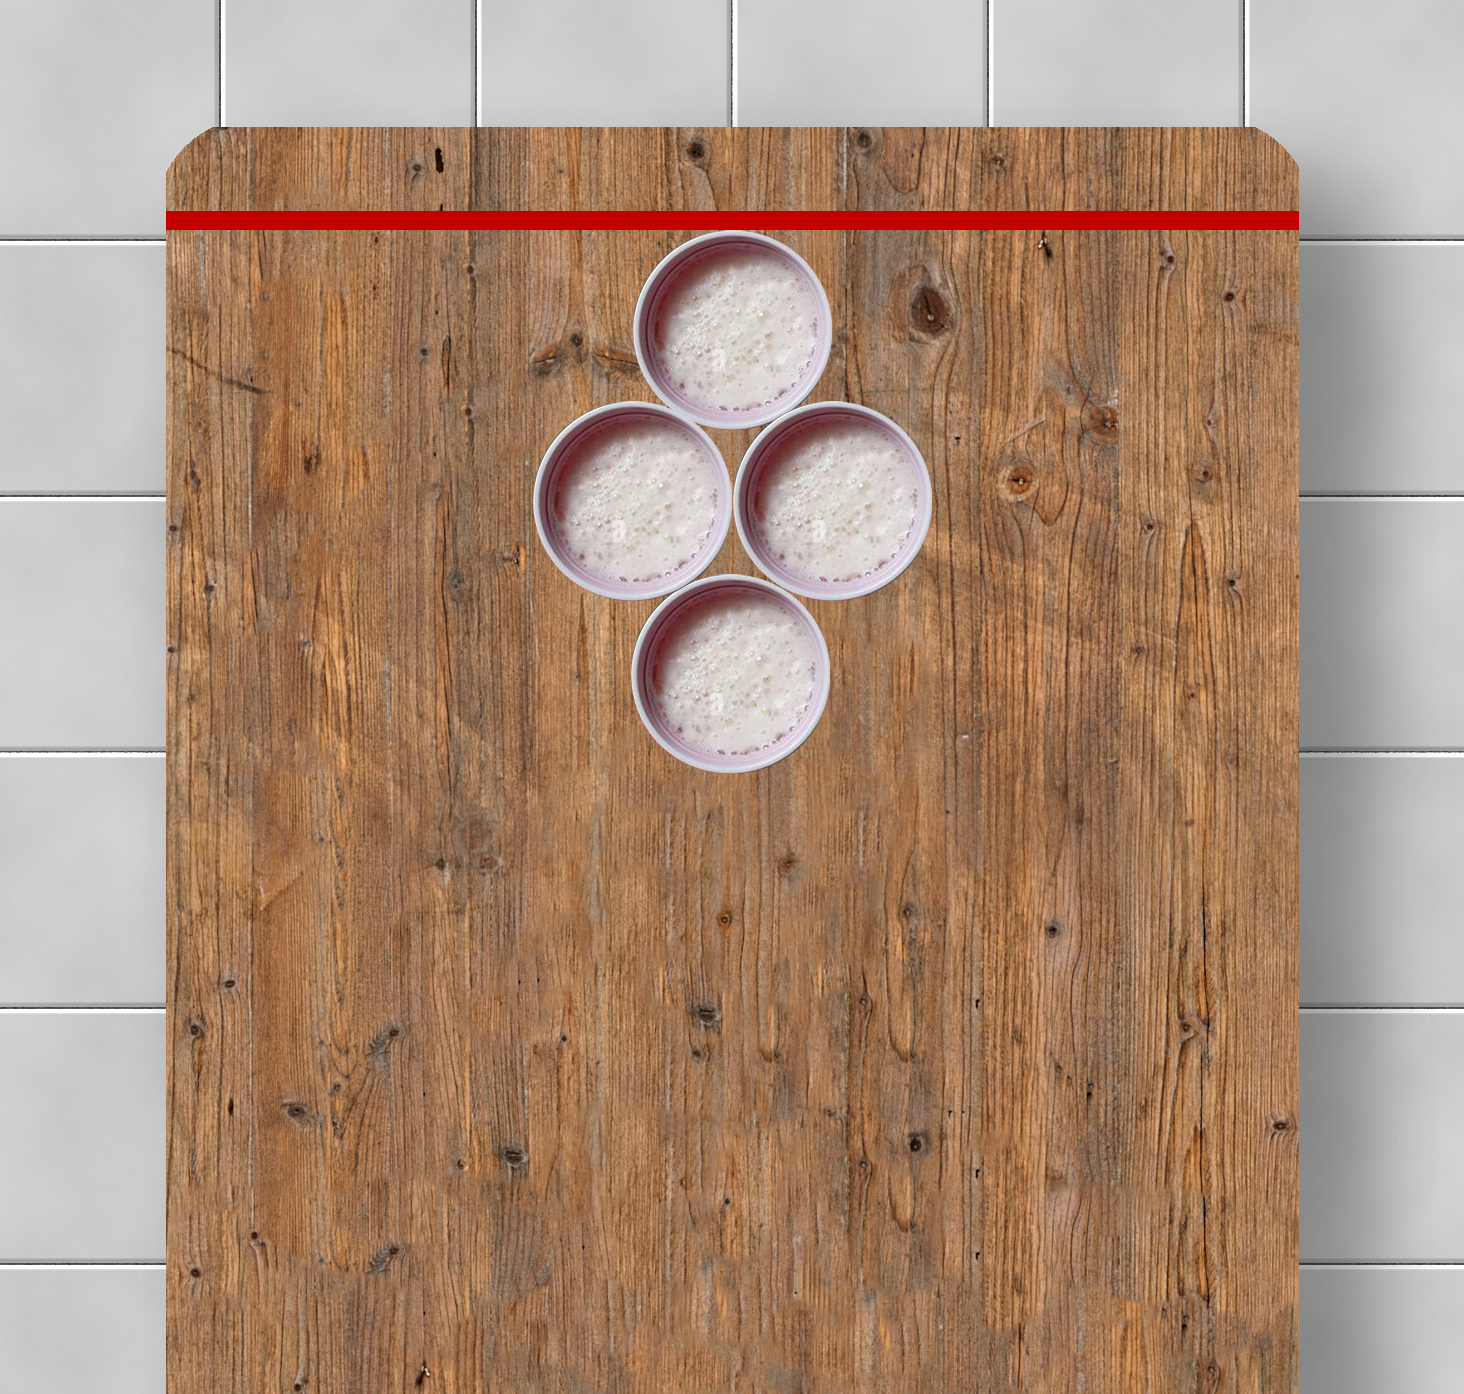
\includegraphics[width=0.434\textwidth]{Grafiken/enge_muschi.png}
    \caption{Die \textit{Enge Muschi}}
    \label{fig:enge-Muschi}
\end{figure}
\begin{figure}[h!]
     \centering
     \begin{subfigure}[b]{0.434\textwidth}
         \centering
         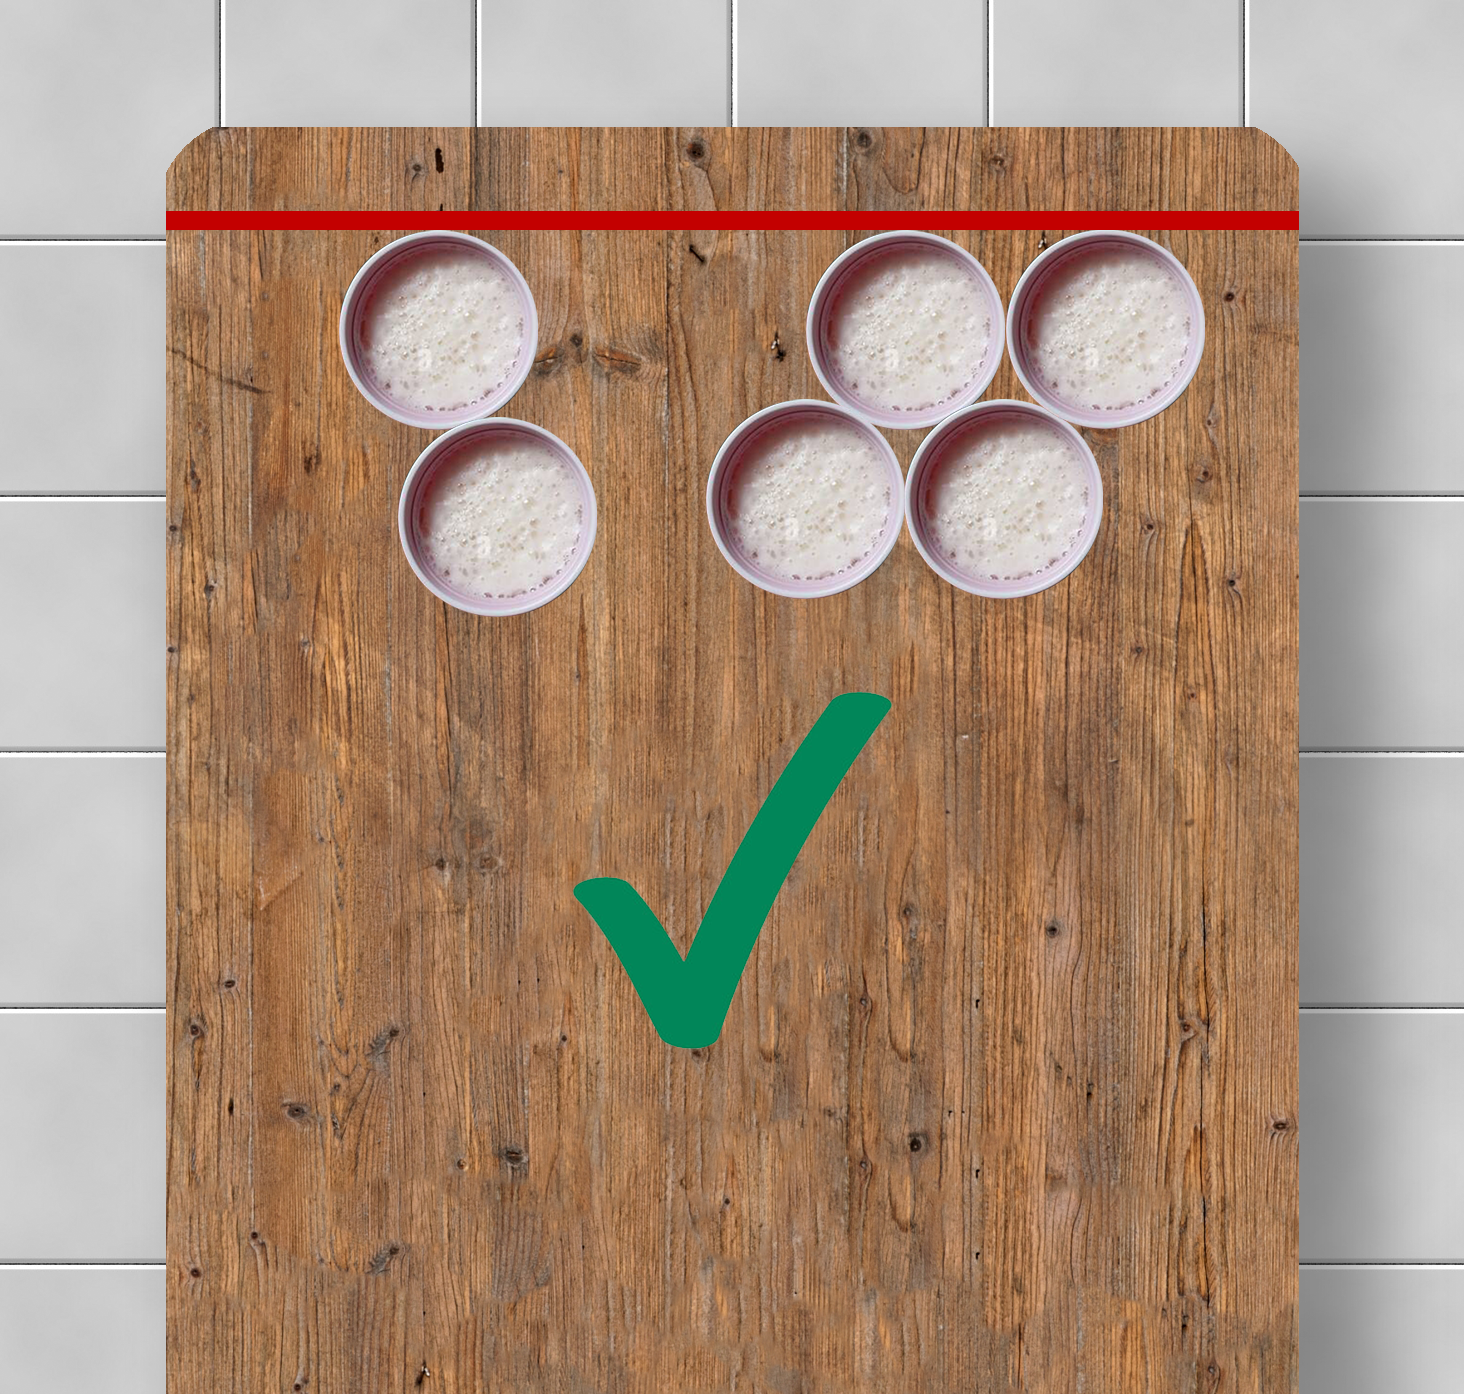
\includegraphics[width=\textwidth]{Grafiken/stellung3.png}
         
    
     \end{subfigure}
     \hfill
     \begin{subfigure}[b]{0.434\textwidth}
         \centering
         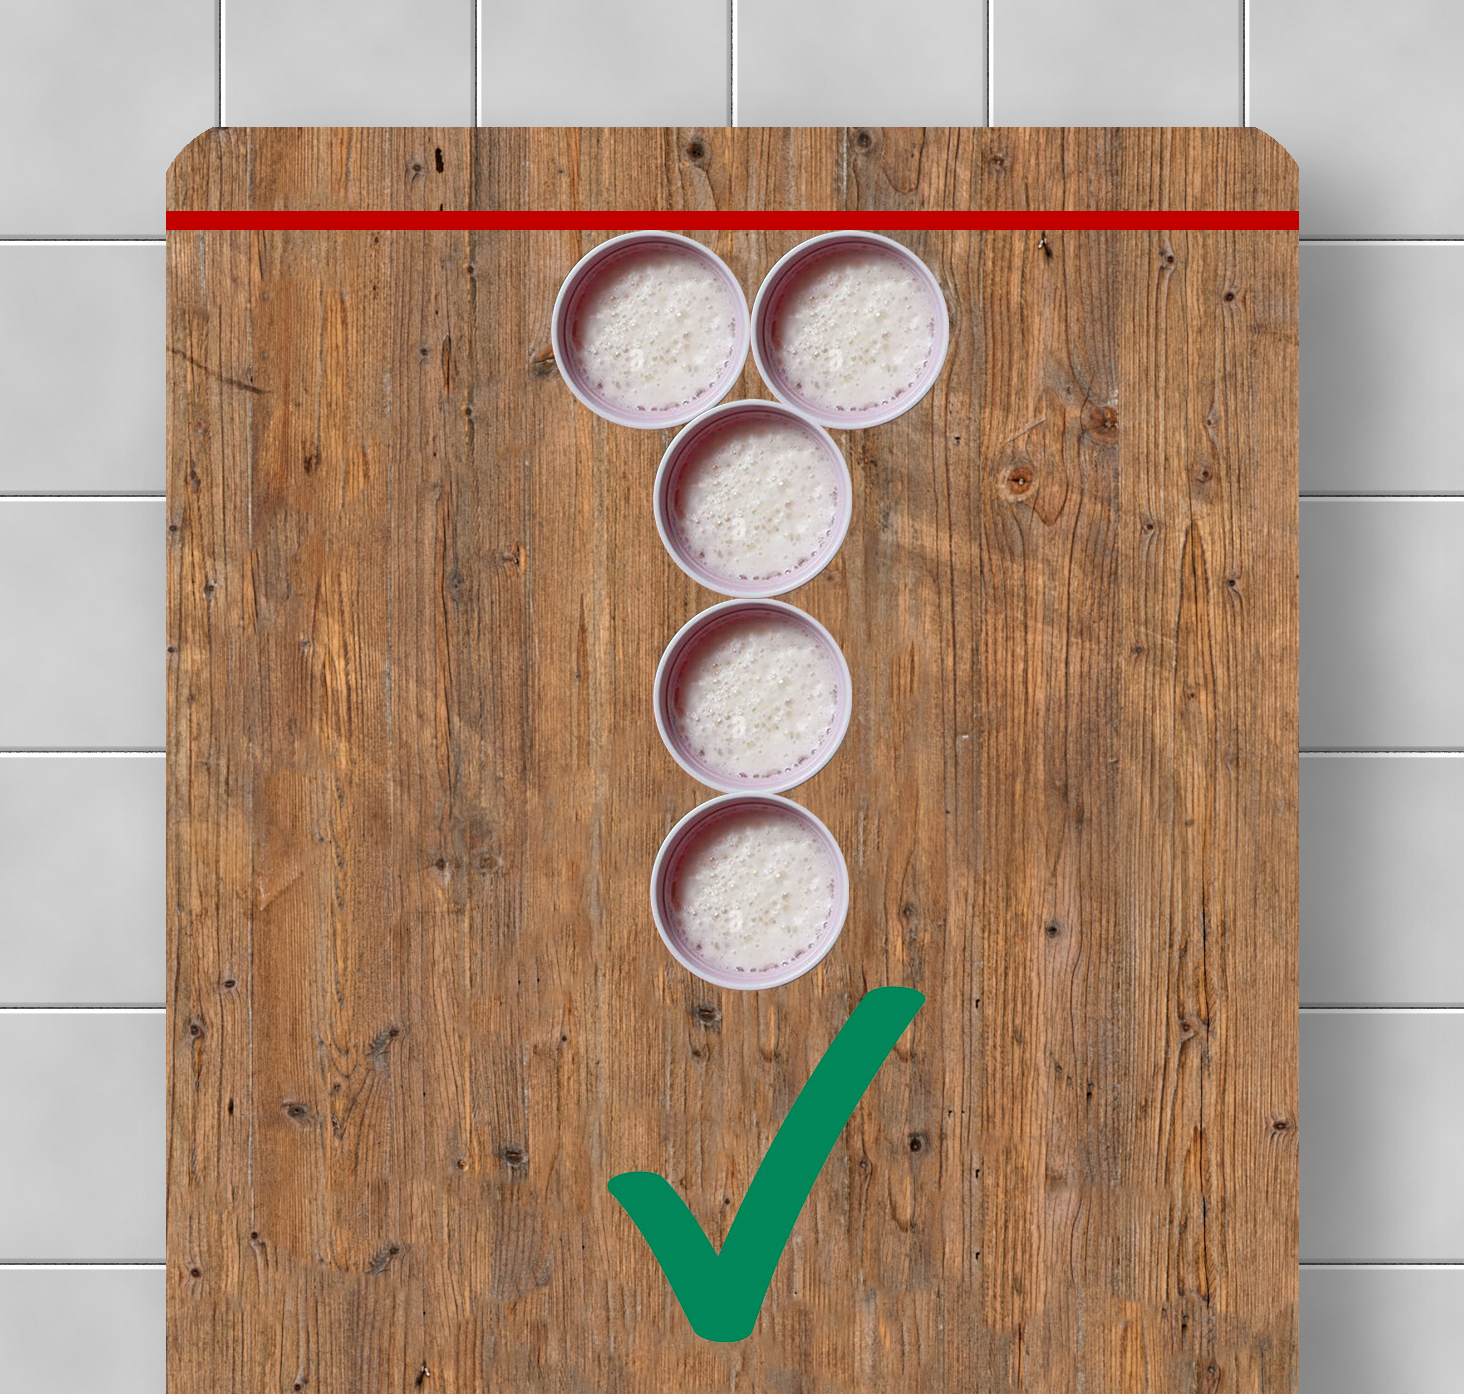
\includegraphics[width=\textwidth]{Grafiken/stellung5.png}
         
     \end{subfigure}
     \hfill
     \begin{subfigure}[b]{0.434\textwidth}
         \centering
         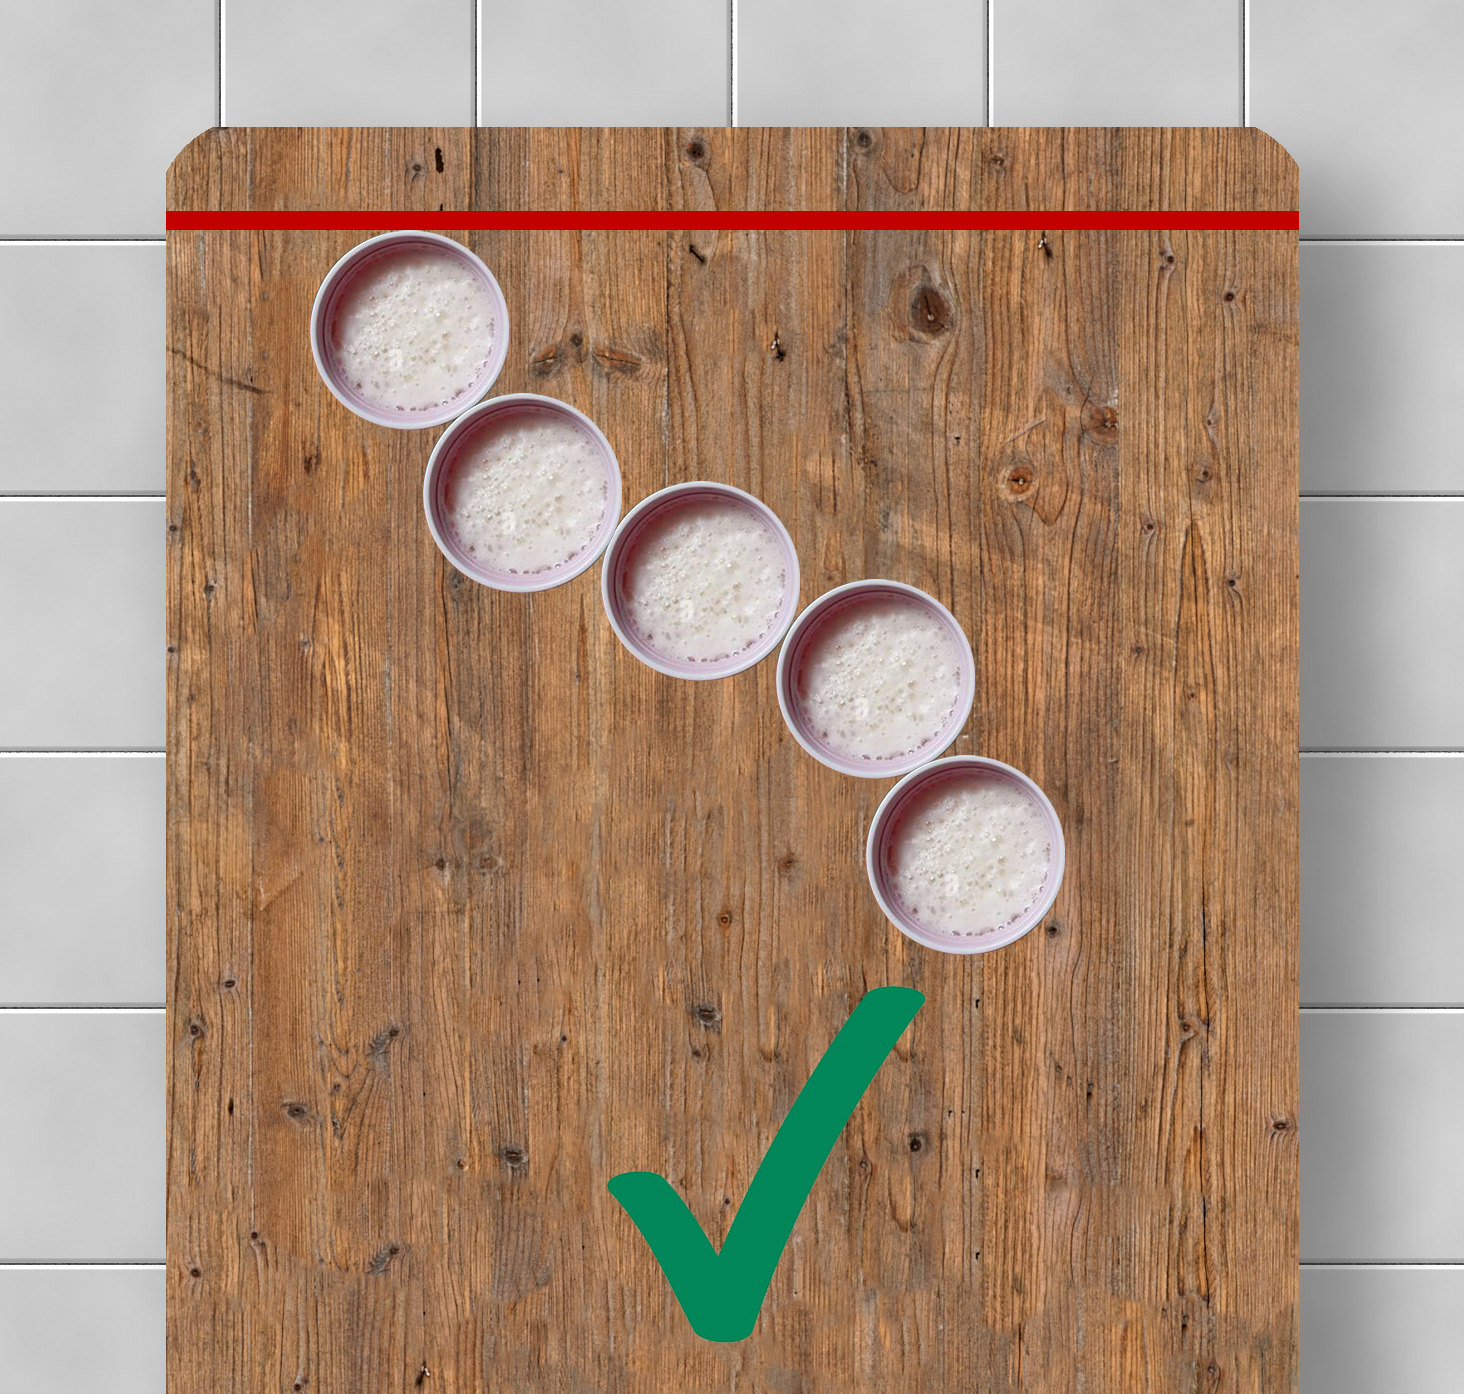
\includegraphics[width=\textwidth]{Grafiken/stellung7.png}
         
     \end{subfigure}
     \hfill
     \begin{subfigure}[b]{0.434\textwidth}
         \centering
         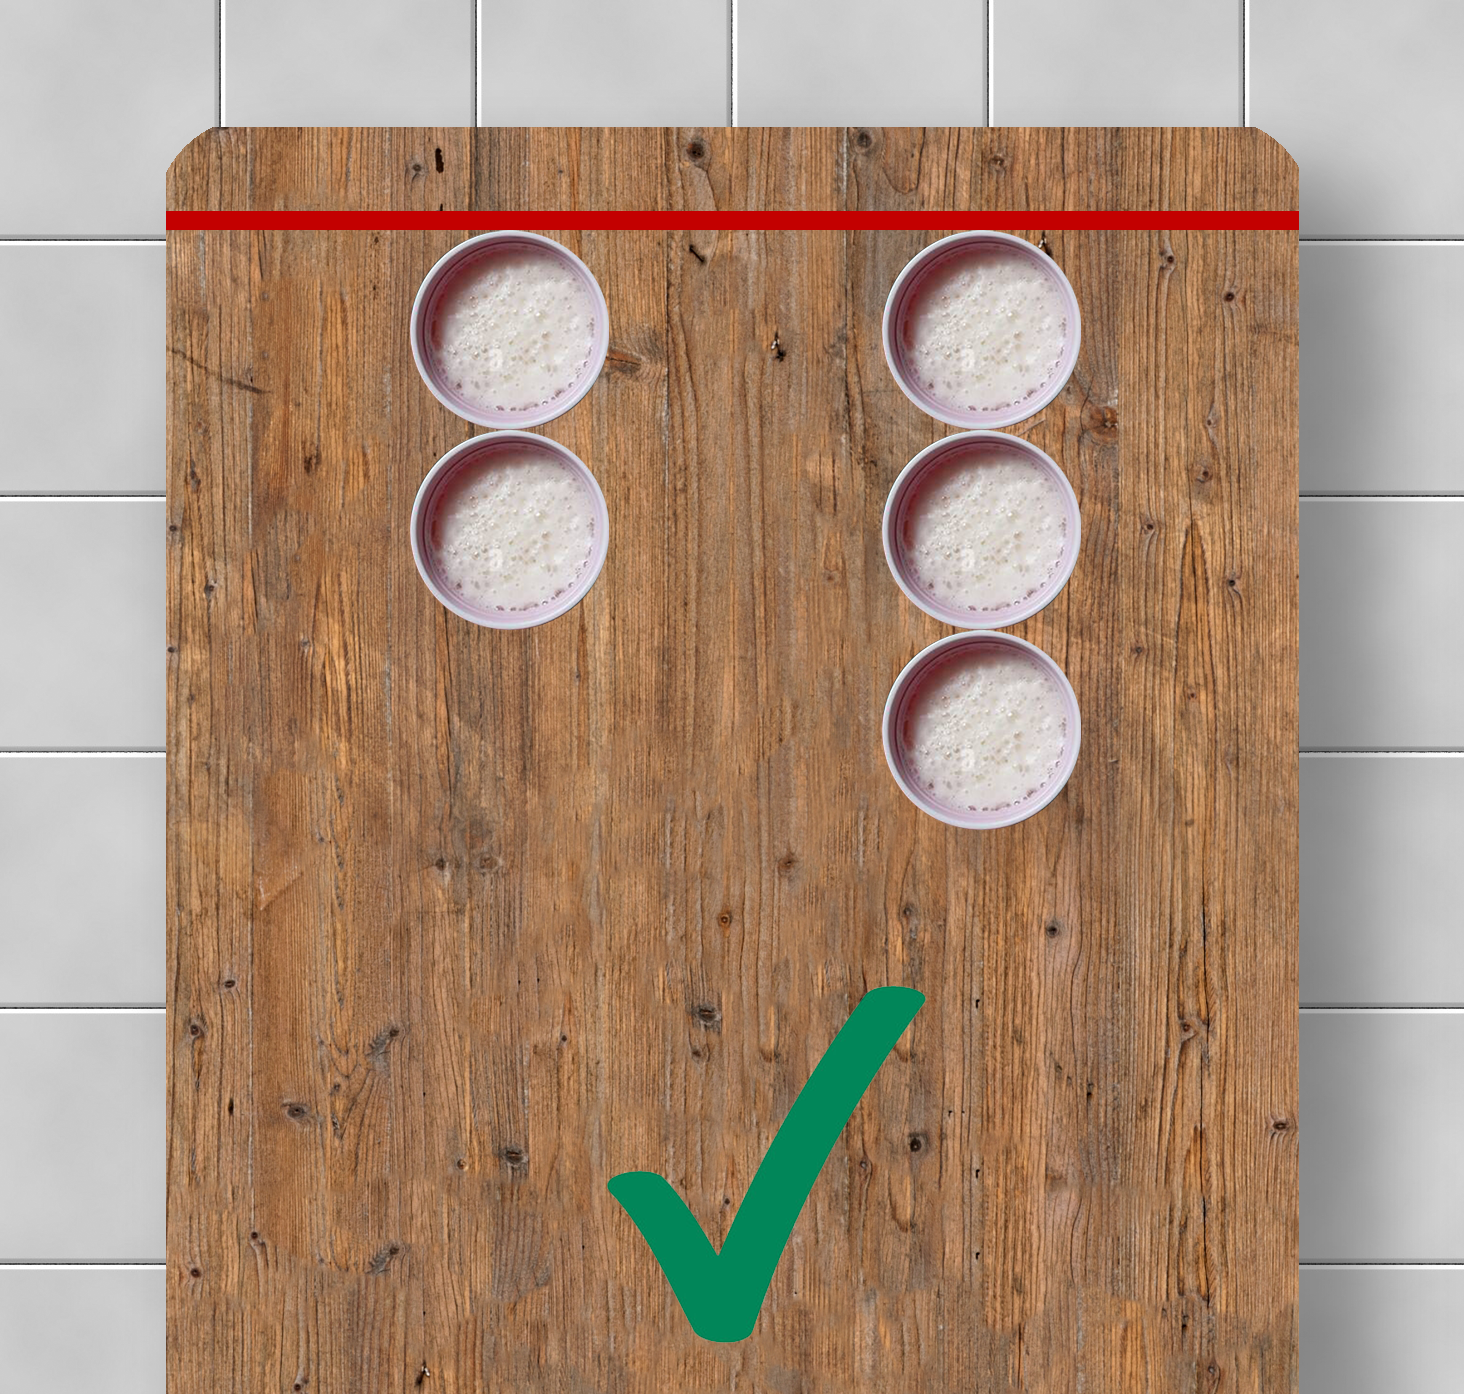
\includegraphics[width=\textwidth]{Grafiken/stellung8.png}
         
     \end{subfigure}
        \caption{Examples for allowed formations}
        \label{fig:beispielezudenerlaubtenStellungen}
\end{figure}
\begin{figure}[h!]
     \centering
     \begin{subfigure}[b]{0.434\textwidth}
         \centering
         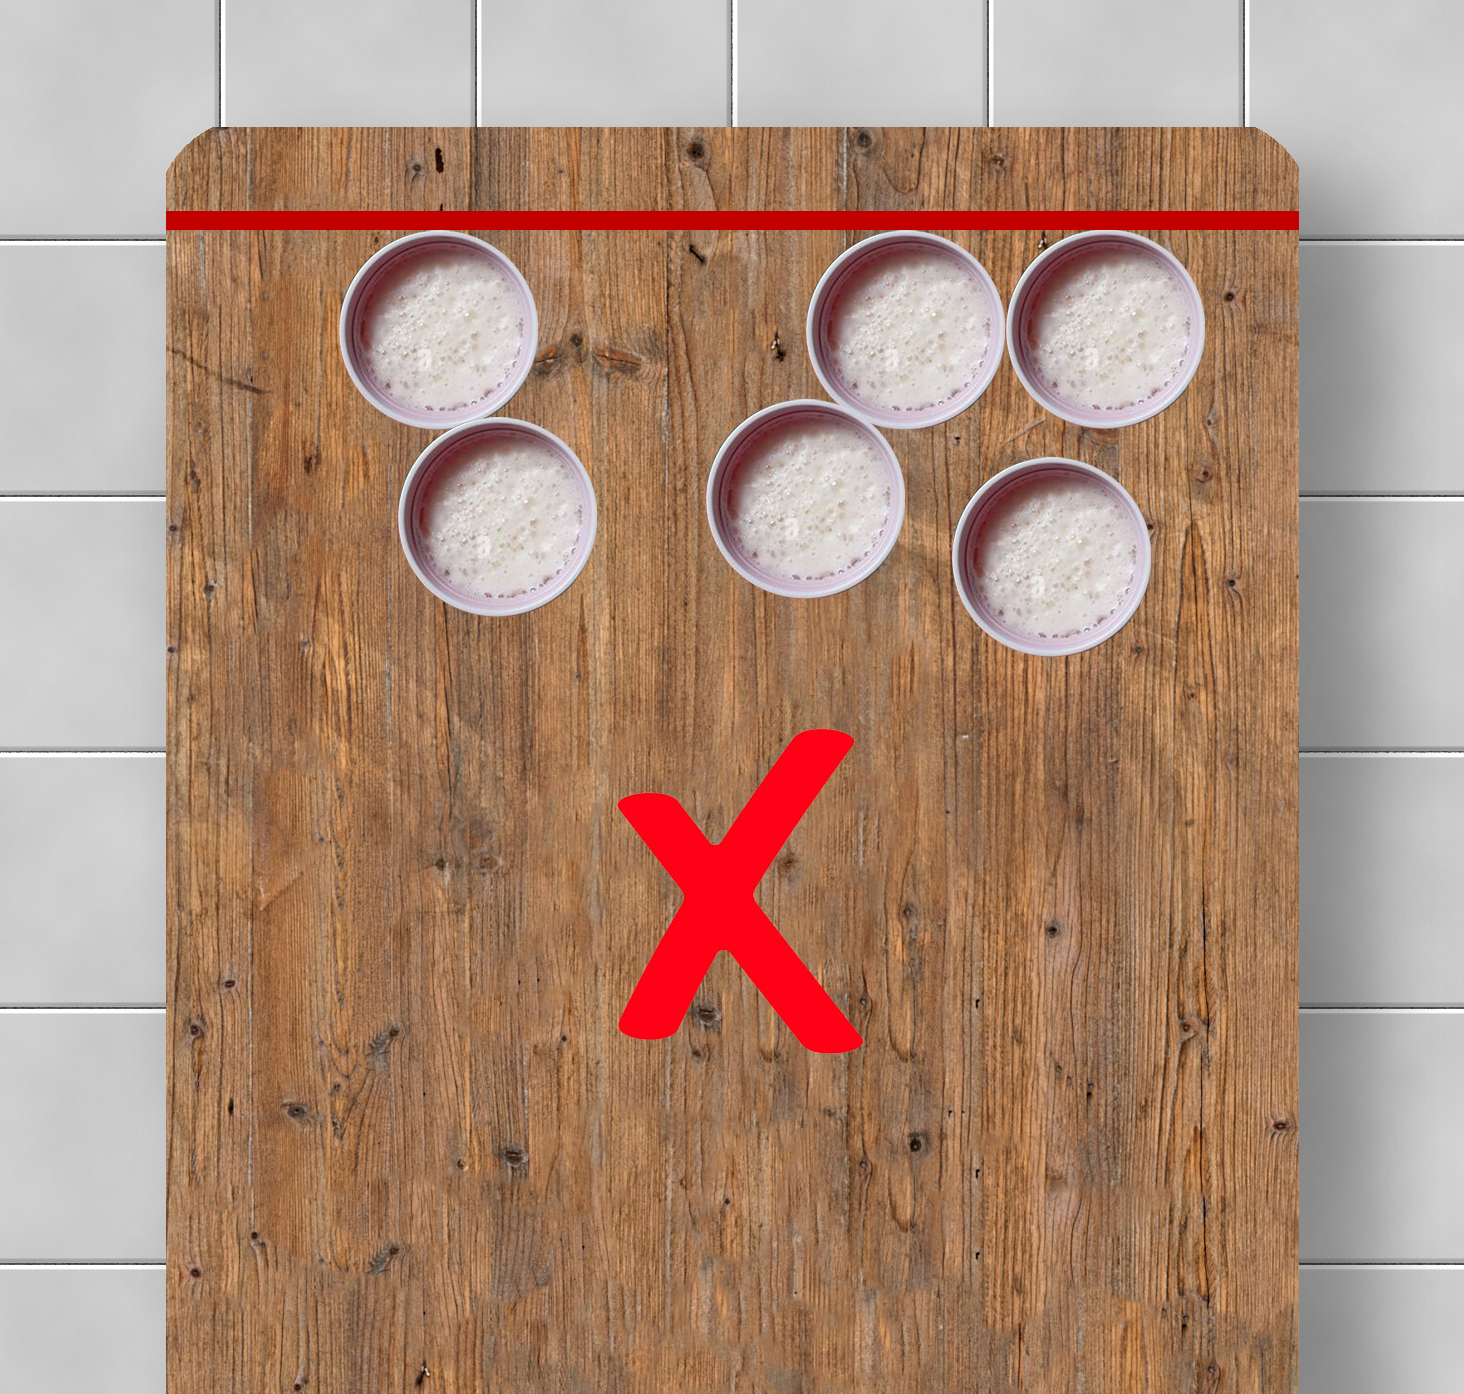
\includegraphics[width=\textwidth]{Grafiken/stellung1.png}
         \caption{the lone cup has no contact with the baseline}
    
     \end{subfigure}
     \hfill
     \begin{subfigure}[b]{0.434\textwidth}
         \centering
         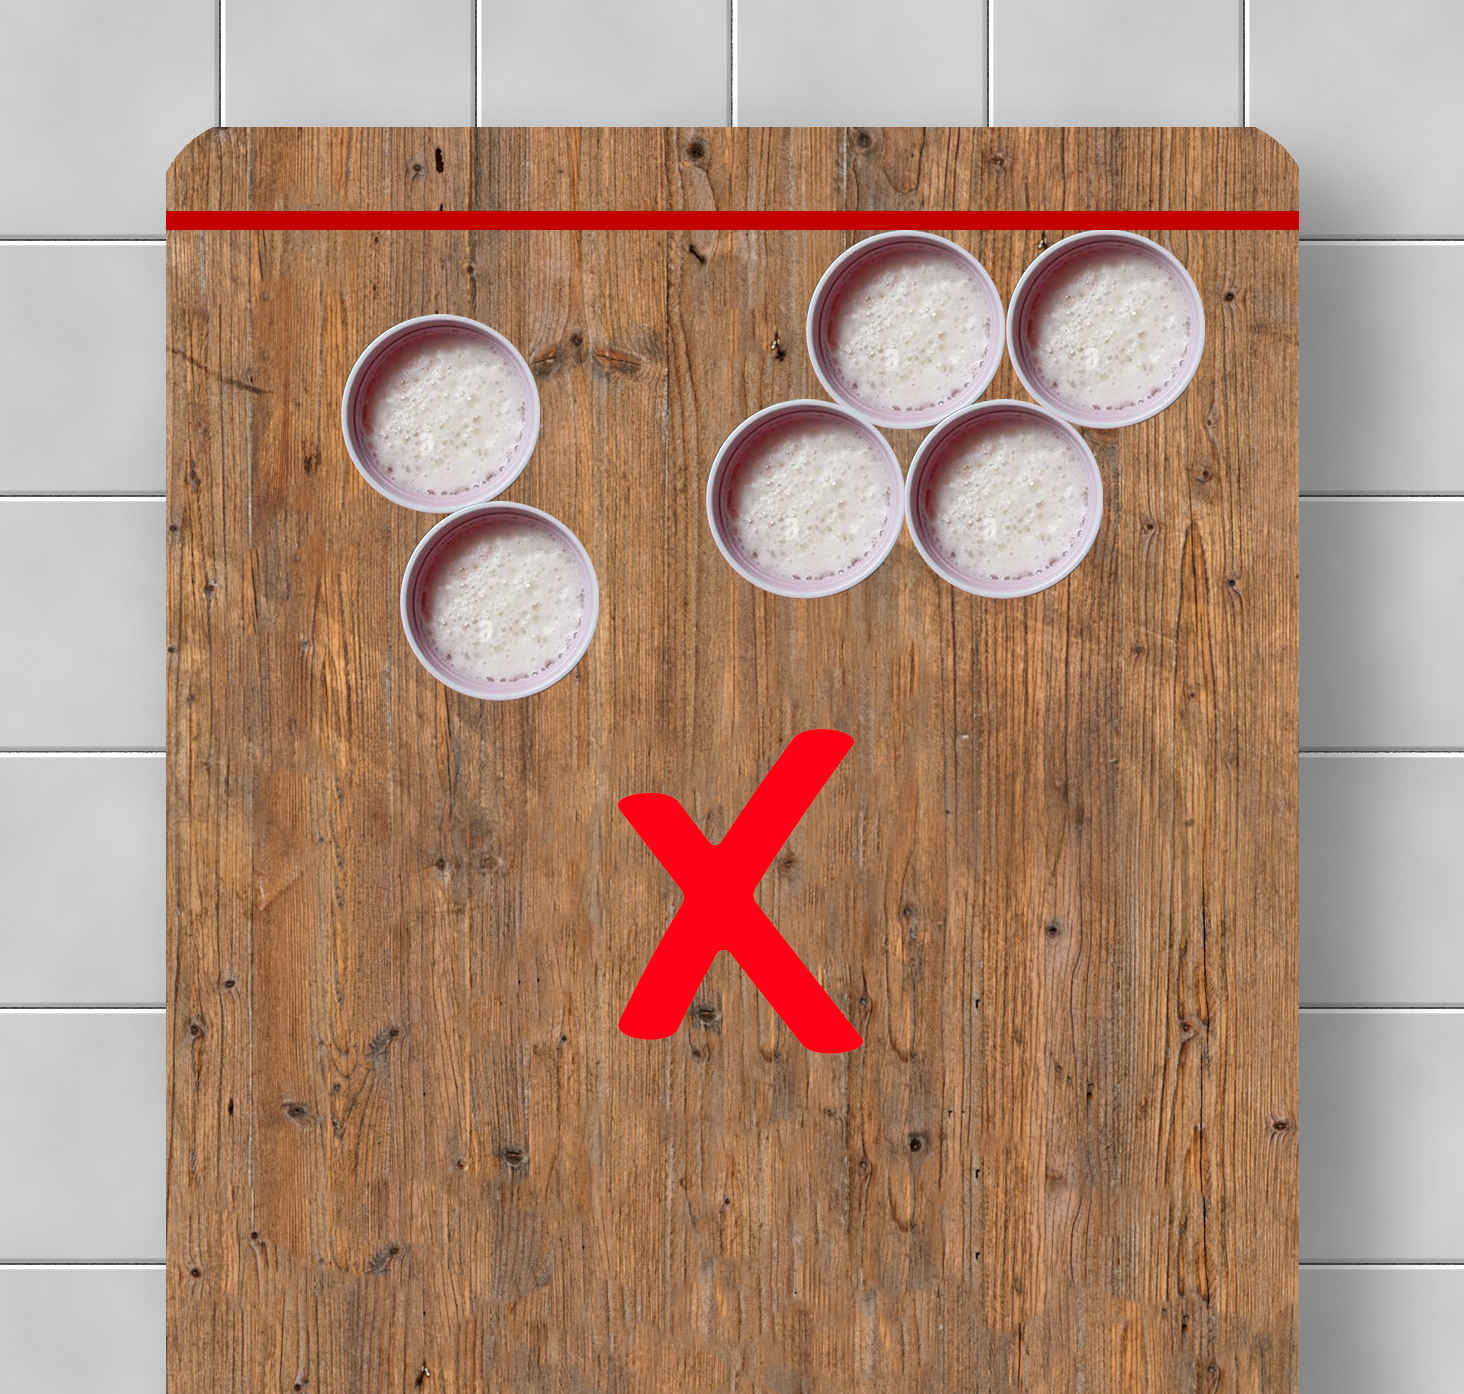
\includegraphics[width=\textwidth]{Grafiken/stellung2.png}
         \caption{the 2 cup group has no contact with the baseline}
     \end{subfigure}
     \hfill
     \begin{subfigure}[b]{0.434\textwidth}
         \centering
         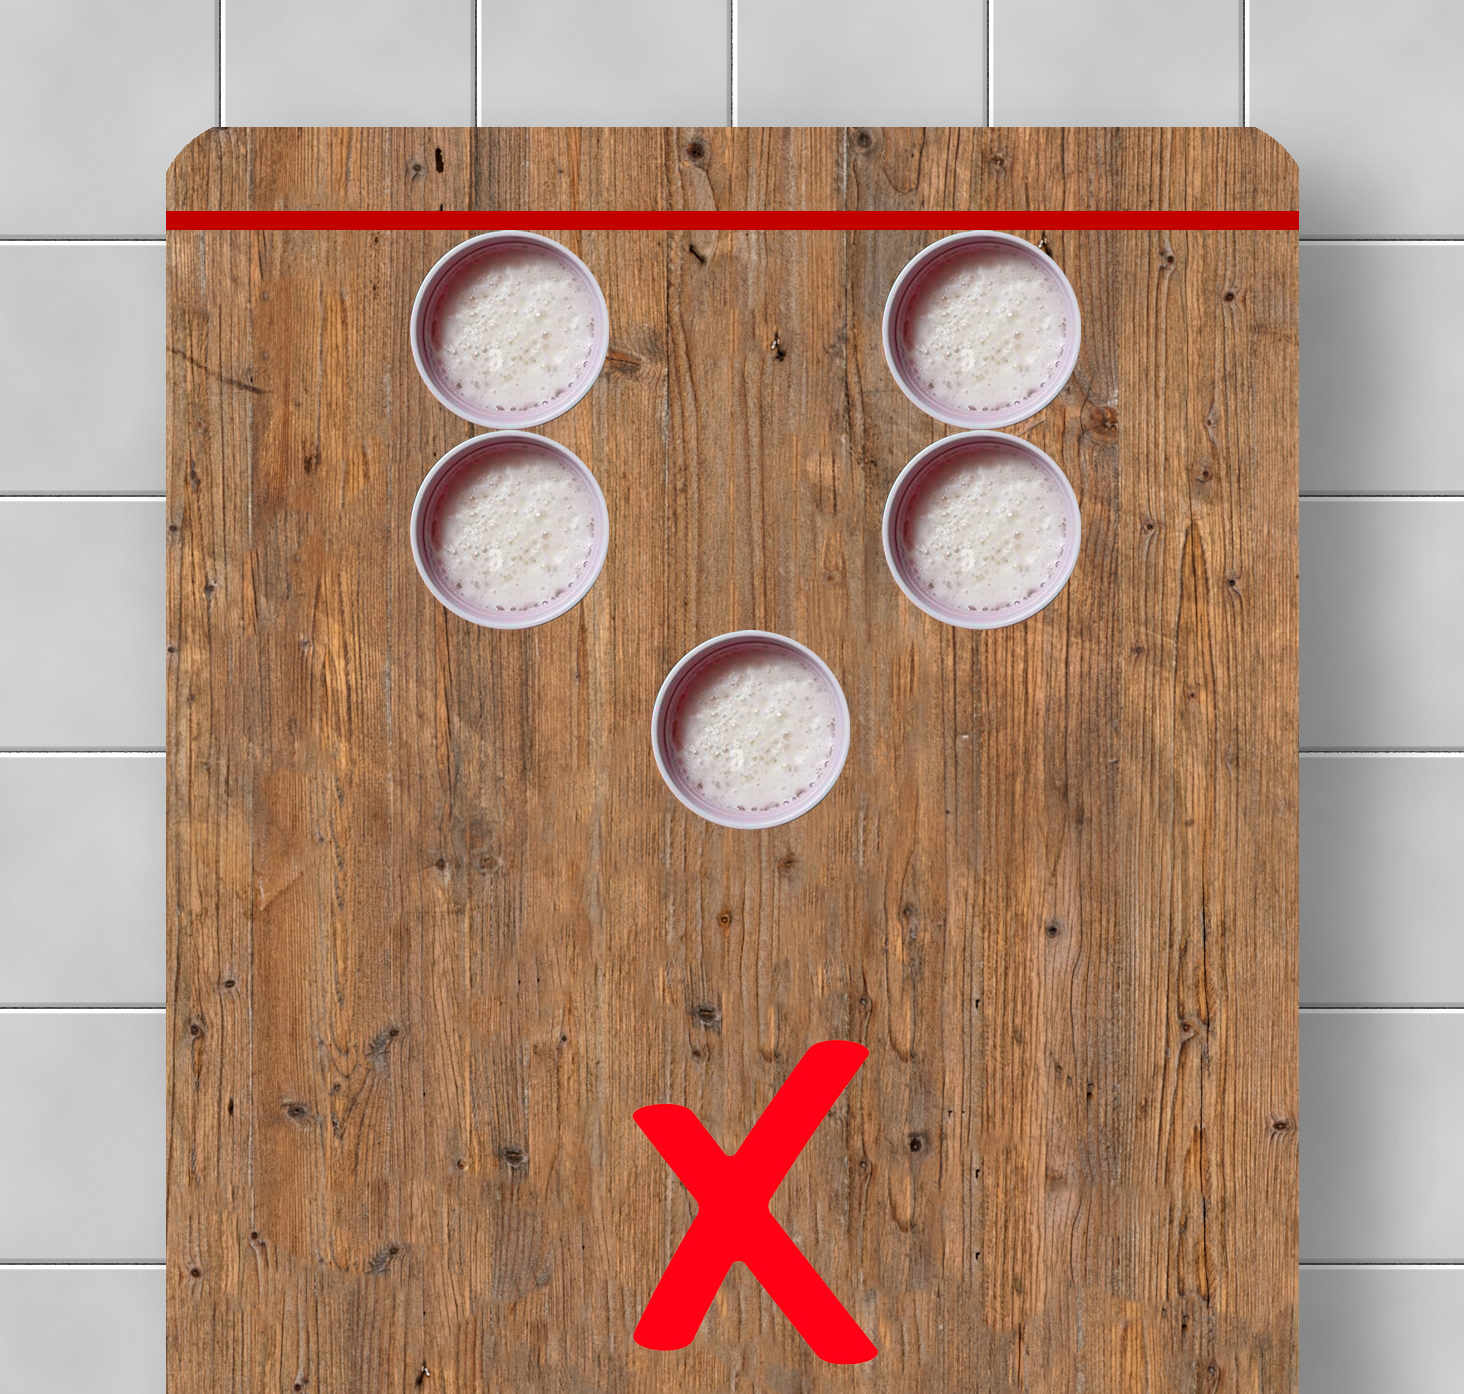
\includegraphics[width=\textwidth]{Grafiken/stellung4.png}
         \caption{the foremost cup has no contact with the baseline}
     \end{subfigure}
     \hfill
     \begin{subfigure}[b]{0.434\textwidth}
         \centering
         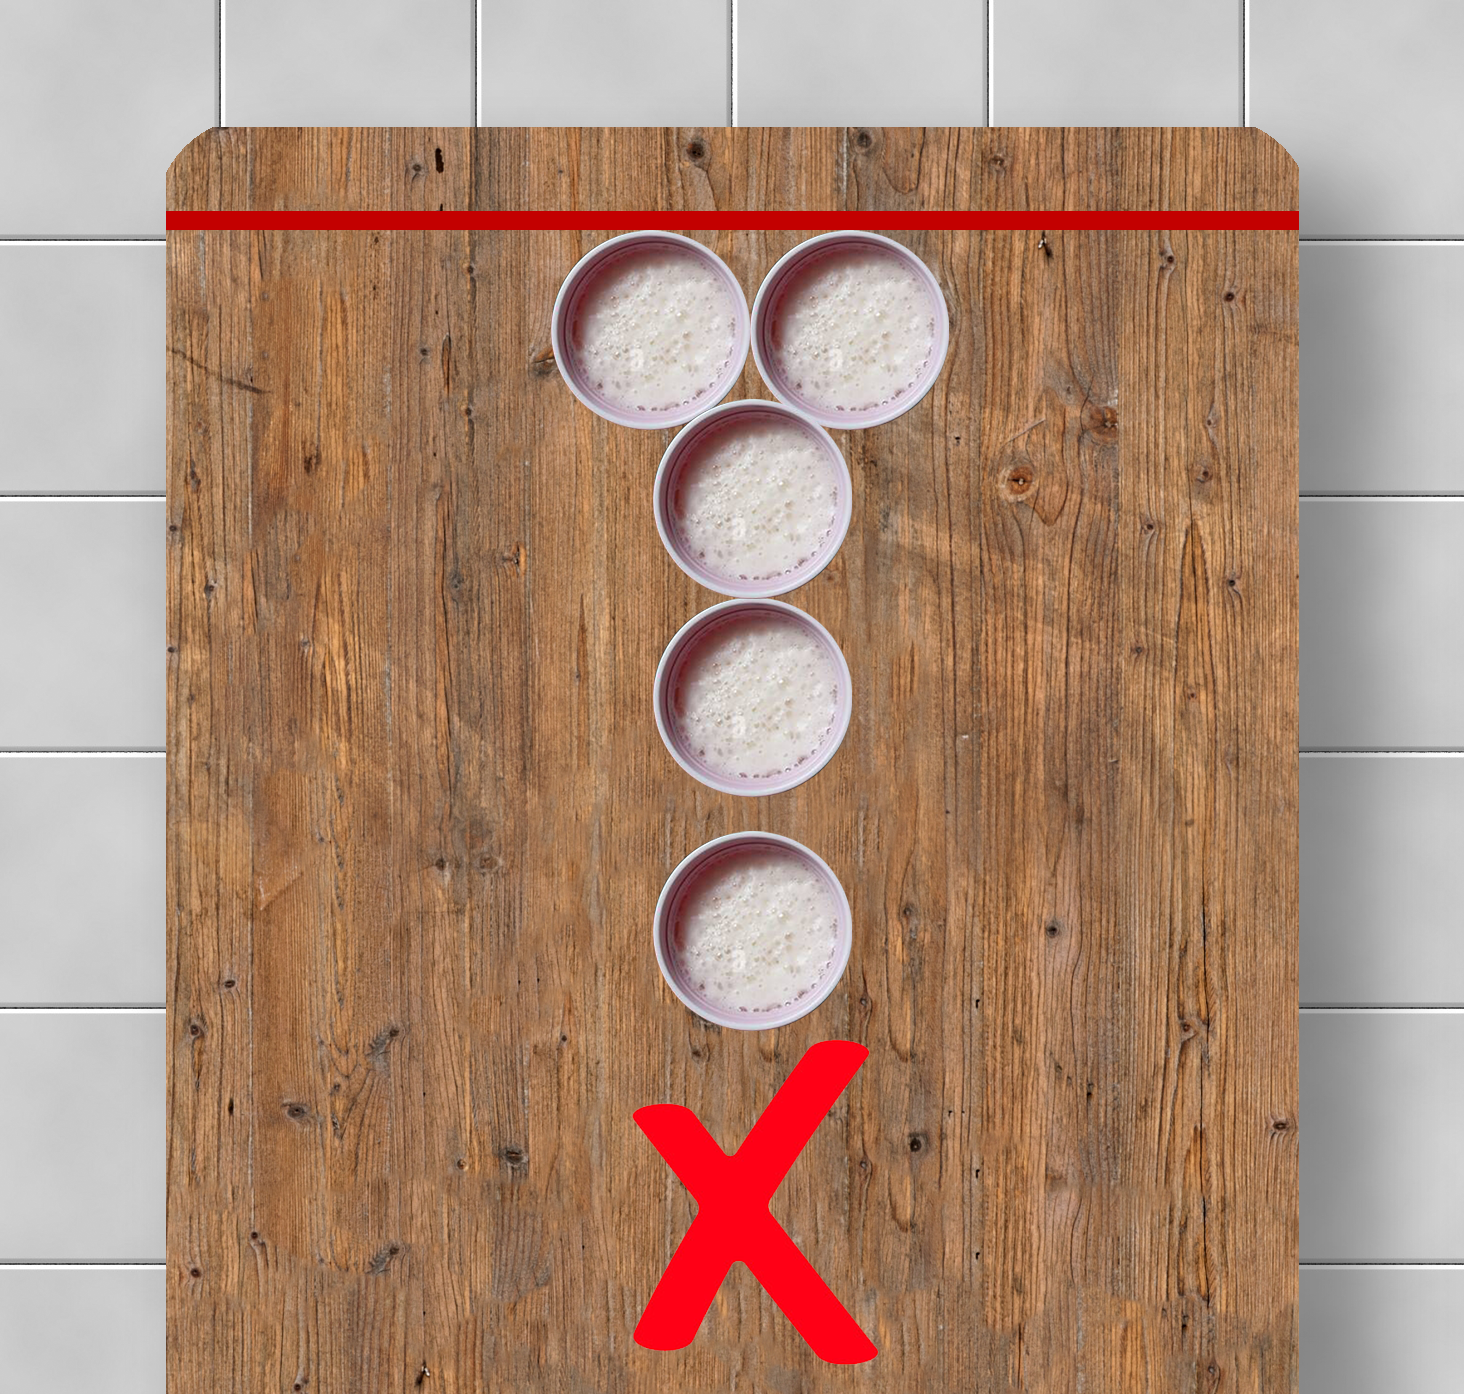
\includegraphics[width=\textwidth]{Grafiken/stellung6.png}
         \caption{even a small gap isnt allowed}
     \end{subfigure}
        \caption{examples for not allowed formations}
        \label{fig:beispielezudennichterlaubtenStellungen}
\end{figure}

After the Rearrangement Phase, the same team continues with the Regular Throw Phase.

\subsubsection{Regular Throw Phase}\label{sec:regular_throw}
Both players of a team may, one after another or simultaneously (as they wish), each perform one Standard Throw.  
After these two throws, the same team proceeds to the BallsBack Phase.

\subsubsection{BallsBack Phase}\label{sec:ballsback}

\paragraph{(1) Starting Conditions:}  
In the previous BallsBack Phase or Regular Throw Phase, both players scored.

\paragraph{(2) Execution:}  
Both players may now each perform one Standard Throw.  
After these two throws, the BallsBack Phase ends, and the starting conditions are checked again to see whether another BallsBack Phase can begin.  
If the conditions are not fulfilled, the same team proceeds to the OnFire Phase.

\subsubsection{OnFire Phase}\label{sec:onfire}

\paragraph{(1) Starting Conditions:}  
At least one player of the active team has three OnFire Stacks (see Section \ref{sec:onfirestacks}).

\paragraph{(2) Execution:}  
One of the players with three OnFire Stacks may perform one Standard Throw.  
If both players of a team have three stacks, the one who threw last performs the throw.  
After this single throw, the OnFire Phase ends, and the conditions for a new OnFire Phase are checked again.  
If they are not fulfilled, the game continues with the Trickshot Phase; if they are fulfilled, the OnFire Phase begins anew.

\subsubsection{Trickshot Phase}\label{sec:trickshotphase}

\paragraph{(1) Starting Conditions:}  
The active team has at least one Trickshot Stack (see Section \ref{sec:trickshotstacks}).

\paragraph{(2) Execution:}  
A team throws as many Trickshots as they have Trickshot Stacks.  
The two team members alternate in throwing.  
Then the Trickshot Phase ends.

After the Trickshot Phase, the other team starts with its Rearrangement Phase.

\subsection{End of the Game}\label{sec:spielende}

The game ends when one of the following conditions occurs:

\begin{enumerate}
    \item The last cup of a team is marked as hit, and they fail to counter (see Section \ref{sec:redemption}).
    \item A measurement finds more than 80 ml in a cup during a complaint (see Section \ref{sec:80ml}).
    \item A Deathcup is scored (see Section \ref{sec:deathcup}).
\end{enumerate}

The following steps are carried out in any order after the game has ended.

\subsubsection{Drinking Remaining Cups}
The losing team must drink the cups still standing on the winner’s side of the table.  
Other people — including members of the winning team — may, out of mercy, help them.

\subsubsection{Naked Mile}\label{sec:nacktemeile}
If a player does not score a single cup during the entire game, she must run a naked mile.  
A score into one’s own cup or during Eye to Eye does not count to avoid the naked mile.  

The route for the naked mile is as follows:  
Start at the front door of the Wal-WG™ apartment, go down the stairs, out the main door, around the fire pit in the upper garden, back inside through the main door, up the stairs to the top, and back down into the Wal-WG™.

Ideally, the run is done completely naked.  
However, if someone would not do it fully naked, she may keep certain items of clothing on.  
If multiple players must run the naked mile, they must do so holding hands.

\subsubsection{Photo}
A photo must be taken of the winning team.  
It must then be sent to a Wal-WG™ member or uploaded via the QR code here/on the wall.



\begin{figure}[htbt]
    \centering
    \includegraphics[scale = 0.1]{Grafiken/bilder}
    \caption{Foto Upload}
    \label{fig:fotoupload}
\end{figure}
\chapter{Further Rules}\label{chap:weitere_regeln}

In the following chapter, all additional rules are listed that apply to the game.  
If a rule is not listed here, it does not apply.

\section{Bomb}\label{sec:bombe}
If both players of a team score in the same round into the same cup, then, in addition to that cup, two more cups are marked as hit.  
Which two additional cups these are is decided by the team whose cups they are.

If the opposing team has four or fewer cups left at the start of that phase, then only one additional cup counts as hit.  
(If only one cup remains, it may also count as double hit.)

To avoid interference during bombs, it is considered good manners to remove the ball from a cup immediately after it was thrown in, before the next throw is made.

\section{Elbow}\label{sec:ellenbogen}
When a player performs a Standard Throw, at the exact moment when the ball leaves her hand, her elbow must be behind her own short edge of the table.  
It is the responsibility of the opposing team to ensure that this rule is followed.  
If they suspect that the elbow was too far forward, it must be discussed whether this was actually the case.  
If so, the throw is invalid and will not be repeated.  
In a disputed situation, the throw may be repeated.

\section{Redemption}\label{sec:redemption}
If a team marks the last cup as hit \( n \) times, the other team must attempt to counter.  
To do so, they start normally with the Rearrangement Phase.  
Now they collect Hits throughout all phases.  
Then there are several cases:

\begin{enumerate}
    \item Exactly \( n \) Hits: counter successful, all cups remain exactly as they are.
    \item More than \( n \) Hits: counter successful, all Hits after the \( n \)-th Hit count normally.
    \item Fewer than \( n \) Hits: counter unsuccessful, the game is lost.
\end{enumerate}

\textbf{Special Case:}  
Team A has one cup left on their side.  
They collect Hits on all of Team B’s cups.  
Team B achieves the counter with the same number of Hits, so Case (1) applies.  
Then an overtime is played.  
This means that both teams must drink their remaining cups.  
Then each team places three new cups in a small pyramid, centered along the baseline, and fills them with half the amount originally used at the start of the ten-cup setup.  
Now a new starting team is determined again (see Section \ref{sec:decidewho}).

\textbf{Clarification:}  
Although this follows directly from the above, the question arose as to what happens if, during the game, a cup is first scored but then more counters occur than needed for overtime.  
One might think that Hits could carry over into overtime.  
That is not the case.  
Overtime only occurs when there is an exact counter.  
In our example scenario, we are therefore in Case (2): the team that first scored the last cup must now counter.

\section{Bounce Shot}\label{sec:aufsetzer}
If a Standard Throw, after leaving the hand, first touches the table and then scores, one additional cup is also marked as hit.  
Which one that is is decided by the team that must drink it.  
As soon as the ball has bounced once, the opposing team may slap it away.

This rule applies only if the opposing team had five or more cups at the start of that phase.

\section{Deathcup}\label{sec:deathcup}
If a cup that a player is currently supposed to drink is scored, then her team immediately loses, except in the following case:  
The opposing team, for any reason, does not have to drink any or all of the cups belonging to the game (for example, if they have water in the cups and drink from bottles).  
A throw during Eye to Eye in overtime is excluded from this rule.

\section{Island}\label{sec:island}
Each player has the right to call “Island” once per game.  
To do this, she must name any island (see Section \ref{sec:whatisanisland} for details on what counts as an island).  
This is only possible when the opponents had five or more cups at the beginning of this Throw Phase.  
She must then identify one single cup that stands alone.  
A cup counts as “standing alone” if, in the current formation, it has no neighboring cups.  
Cups that have shifted slightly still count as neighbors.  

If she scores her next throw into the declared island cup, that cup counts as hit, and one additional cup is also marked as hit.  
The team that must drink decides which one that is.  

However, if any other cup is scored, it does not count as scored.  
(This also applies in particular if a Deathcup is scored; see Section \ref{sec:deathcup}.)

\subsection{What Is an Island?}\label{sec:whatisanisland}
An island is a landmass completely surrounded by water.  
It does not have to be a country — the name of the island itself counts.  
Countries where the island has no separate name also count (for example, Iceland).  
Australia also counts as an island.  
The name of an island group counts as well (for example, Indonesia).  
A country that lies on an island but is not the island’s name itself does not count (for example, Haiti — the correct designation here would be Hispaniola).\\
Fantasy islands are allowed. In this case the liquid surrounding mustn't be water.

\section{Last Cup}\label{sec:letzter}
For the last cup to count as hit, it must be scored.

\section{Bitchcup}\label{sec:bitchcup}
This rule takes effect starting with the first Throw Phase.  
If a player scores her team’s first score into a Bitchcup (see Section \ref{chap:spielaufbau}), she must take off or pull down her pants — her choice.  
(If she is not wearing pants, she must remove the outermost layer of clothing that covers her legs.)  
She may put her pants, or whichever item she removed, back on once she scores the next cup of the opponents.  

This rule, like the Naked Mile (see Section \ref{sec:nacktemeile}), is not an absolute obligation — if someone feels uncomfortable undressing, she does not have to do it.

If at the end of the game the pants are still down, they must remain down until, in a following game, she scores another cup.  
If in that following game the Bitchcup is scored again, the topmost layer of clothing on the upper body must be removed.  
This removal is also not mandatory.  
If the player was already naked when she scores the Bitchcup, she must instead perform a spontaneous dance routine.

\section{Fingering / Blowing}\label{sec:fingernblasen}
If a cup is scored, the throw cannot be rendered invalid by fingering the ball out or blowing it out.

\section{80 ml}\label{sec:80ml}
Every player has the right, at any time, to challenge the fill level of a cup belonging to the opposing team that has not yet been drunk and is not currently being drunk.  
This can only be done with cups from which no liquid has unintentionally spilled.  
If, after measurement, it turns out that the cup contained less than 80 ml, it must be drunk.  
However, if it contained 80 ml or more, then the challenger’s team immediately loses the game.  
This verification is carried out using the Wal-WG™’s own Beer Pong scale.  
The empty weight of one of the hard-plastic cups is:

\section{Space Laser}\label{sec:weltraumlaser}
Anyone who scores a Space Laser gets her own DIN A3 framed picture on the wall.  

A Space Laser is a throw from the window side where the ball, thrown with great force, hits the top edge of the door and bounces directly into the cups on the door side.

\section{Touching the Ball in Flight}\label{sec:ballflug}
If a player touches the opponent’s ball while it is in flight, and that ball does not result in a score, her team must drink one cup of their choice — provided the following conditions are all met:

\begin{enumerate}
    \item The touch occurred before the ball crossed her own short table edge.
    \item The throw was roughly on course to hit a cup.
    \item The opponent team was not throwing one normal throw and one bounce shot simultaneously.
    \item The deflected ball was not a bounce shot.
\end{enumerate}

\textbf{Special Case:}  
If the touched ball was aimed at only one remaining cup:  
since the last cup must always be scored, it cannot be chosen as the penalty cup.  
Therefore, the opposing team receives two additional Standard Throws.  
Furthermore, this counts as unsportsmanlike conduct and may lead to disqualification — especially if the throw was on a good trajectory.

This rule is weaker than Section \ref{sec:ballaufbecher_springen}.

\section{Community Cup}\label{sec:communitycup}
If a ball, in any way but not intentionally, lands in one of the empty cups placed on the edge of the table, then all spectators must take a sip of their drink.

\section{Moving Cups forward}\label{sec:bechervorstellen}
To prevent cups from constantly falling to the floor, each team has the right to move its cups that are close to the edge forward so that they still touch the baseline.  
This may be done at any time, except when an opponent is already in the act of throwing.

\section{Touching Cups}\label{sec:becherberuehren}
Unless performing one of the following actions, no player may touch a non-empty cup during the game:

\begin{enumerate}
    \item Rearranging (see Section \ref{sec:umstellphase})
    \item Presenting (see Section \ref{sec:bechervorstellen})
    \item Removing the ball from a cup
    \item Drinking (see Section \ref{sec:bechertrinken})
    \item Catching or restacking a cup that has fallen from the table (see Section \ref{sec:treffer})
    \item Setting up and filling the pyramid for overtime
\end{enumerate}

If a player touches a cup anyway, and it was one of her own cups, she must drink it.  
If it was an opponent’s cup, she must drink a self-chosen cup from her own side.

\section{Airball}\label{sec:airball}
If a Standard Throw touches neither the tabletop nor anything else located on the table before being touched by an opposing player, it counts as an Airball.  
In this case, Section \ref{sec:ballflug} must be carefully observed.

\section{Stacks}\label{sec:stacks}
Stacks can be collected by a player or by a team.  
There are three types of stacks: Trickshot Stacks, OnFire Stacks, and OnIce Stacks.

\subsection{Trickshot Stacks}\label{sec:trickshotstacks}
If a player throws an Airball, there are two options:

\begin{enumerate}
    \item The opposing team receives one Trickshot Stack.
    \item Both teams agree to cancel it out.  
    This is only possible if the throwing team already has at least one Trickshot Stack.  
    In that case, the throwing team loses one Trickshot Stack, and the opponents receive none for this Airball.
\end{enumerate}

At the end of a team’s Trickshot Phase, all of its Trickshot Stacks are reset to 0.

\subsection{OnFire Stacks}\label{sec:onfirestacks}
For every scored Standard Throw or Trickshot, a player receives one OnFire Stack  
(throws during Eye to Eye do not count).  
If she misses a throw during the Regular Throw Phase or the OnFire Phase, all of her OnFire Stacks are reset to 0.

\subsection{OnIce Stacks}\label{sec:onice}
For every Airball, a player gains one OnIce Stack.  
A player’s OnIce Stacks are reset to 0 either when she makes a Standard Throw / Trickshot that is not an Airball,  
or when a Calming Cup (see Section \ref{sec:nervenbecher}) is drunk.

\section{Calming Cup}\label{sec:nervenbecher}
If a player has three OnIce Stacks, she must drink one cup of water to calm her nerves.  
Afterward, her OnIce Stacks are reset to 0.

\section{Obstruction}\label{sec:behinderung}
It is forbidden to physically obstruct an opponent during her throw.

\section{Ball on Cup}\label{sec:ballaufbecher}

\subsection{Staying Put}\label{sec:ballaufbecher_liegen}
If, during a Standard Throw or Trickshot, the ball remains resting on a team’s cups without falling in, that counts as one scored cup.  
The team on whose side it lies may choose which cup counts as scored.

\subsection{Bouncing}\label{sec:ballaufbecher_springen}
If a ball bounces on a team’s cups, that team may knock it away without consequence.  
This rule overrides Section \ref{sec:ballflug}.

\appendix
\part {Anhang} \label{part:anhang}
\chapter{Patch Notes}\label{chap:patchnotes}
This section lists all the changes made from the second to the third edition.  
It begins with those that apply throughout the entire book, followed by all remaining ones from front to back.  
Corrections of commas or rewordings that only improve readability without changing the rules are not listed.

\begin{itemize}
    \item Instead of Wal-WG or just WG, it now consistently says Wal-WG\texttrademark.
    \item The generic masculine form has been replaced with the generic feminine form.
    \item Cross-references to other rules are now more consistent.
    \item The section previously titled “Introduction” is now correctly called “Preface,” and several additions and changes have been made.
    \item It is now written down (at least indirectly) which cups count as belonging to a team (Section \ref{sec:bechertrinken}).
    \item The Guest Throw has been officially added under Trickshot (Section \ref{sec:trickshot}).
    \item Teams of any size are now allowed (Section \ref{sec:teameinteilung}).
    \item A new section was added before the game begins, in which each team decides whether to rearrange at even or odd cup counts (Section \ref{sec:geradeungerade}).
    \item The Rearrangement Phase was adjusted so that rearranging is also possible at odd cup counts (Section \ref{sec:umstellphase}).
    \item The images of possible cup formations were updated (Figures 3.3 and 3.4).
    \item It is now explicitly stated that the OnFire Phase continues when a hit occurs (Section \ref{sec:onfire}).
    \item The Guest Player rule has been moved from the Trickshot Phase to the Trickshot definition (Section \ref{sec:trickshot}).
    \item In the Naked Mile rule, it is now clear that a score into one’s own cup or during Eye to Eye does not count (Section \ref{sec:naktemeile}).
    \item An additional clarification for drunk players was added to Redemption (Section \ref{sec:redemption}).
    \item It is now stated that a player must name an actual island when calling Island, with a clear definition (Section \ref{sec:island}).
    \item It is now clear what happens if the Bitchcup is scored while already naked (Section \ref{sec:bitchcup}).
    \item The measuring method and the empty weight of a cup have been added (Section \ref{sec:80ml}).
    \item The timing of a touch now matters when slapping a ball away without a bounce — this fixes the previous contradiction between the Bounce Shot and Slap Away rules (Section \ref{sec:ballflug}).
    \item The Airball now has its own section and a clearer definition (Section \ref{sec:airball}).
    \item The OnFire Stacks are better defined (Section \ref{sec:onfirestacks}); a third form of stack, OnIce Stacks, has been introduced (Section \ref{sec:onice}).
    \item The Calming Cup has been introduced (Section \ref{sec:nervenbecher}).
    \item The cases for when the ball stays on or bounces off the cups are now explicitly described (Section \ref{sec:ballaufbecher}).
\end{itemize}
\chapter[List of Figures]{List of Figures}\label{chap:Abbildungsverzeichnis}
\listoffigures
\chapter[Request for rulechanges]{Request for rulechanges}\label{chap:antrageaufregelanderung}
The following pages provide space for requests for rule changes.
Please describe precisely what should be changed, how, and why.\\ \newpage
 \newgeometry{total = {4in, 7in}}
\neueregel
\neueregel
\neueregel
\neueregel
\neueregel
\neueregel
\neueregel
\neueregel
\neueregel
\neueregel
\neueregel
\neueregel
\neueregel
\restoregeometry
\chapter{Links}\label{Links}
\begin{figure}
    \centering
    
\includegraphics[scale = 0.1]{Grafiken/Bierpongregeln}
    \caption{\\If you want to become a great Wal-WG\texttrademark\ Beer Pong lawyer, you can download the PDF of the rulebook here.}
\end{figure}
\begin{figure}
    \centering
    
\includegraphics[scale = 0.1]{Grafiken/Elo.png}
    \caption{\\The ranking list in the Wal-WG\texttrademark, record keeping starting on September 23, 2025.}
\end{figure}
\begin{figure}
    \centering
    
\includegraphics[scale = 0.1]{Grafiken/english.png}
    \caption{\\English rulebook}
\end{figure}
\begin{figure}
    \centering
    
\includegraphics[scale = 0.1]{Grafiken/Bilder.png}
    \caption{\\The upload link for all images.}
\end{figure}

\end {document}